% A reference architecture: the interface talks, the models think, plain text remembers.
% ---------------------------------------------------------------------------
% style.tex --- shared preamble for every figure in book/figures/tikz/
%
% One style for all figures: Latin Modern, thin black lines, a light grey
% fill, and one accent colour used only to mark what is untrusted or wrong.
% Build with scripts/build_figures.sh; see book/figures/README.md.
% ---------------------------------------------------------------------------
\documentclass[tikz,border=6pt]{standalone}
\usepackage[T1]{fontenc}
\usepackage{lmodern}
\usetikzlibrary{arrows.meta,positioning,shapes.geometric,calc,fit,backgrounds}

\hyphenpenalty=10000   % short lines in boxes: ragged, never hyphenated

\definecolor{lightgrey}{gray}{0.92}
\definecolor{accent}{HTML}{9B2D20}

\tikzset{
  every picture/.style={
    line width=0.6pt,
    font=\small,
    >={Stealth[length=5pt,width=4pt]},
    node distance=14pt and 24pt,
  },
  % shapes
  box/.style={draw, rectangle, inner xsep=8pt, inner ysep=5pt,
              minimum height=22pt, align=center},
  grey/.style={box, fill=lightgrey},
  rounded/.style={box, rounded corners=9pt},
  decision/.style={draw, diamond, aspect=2.4, inner sep=1.5pt, align=center},
  group/.style={draw, dashed, rounded corners=5pt, inner sep=7pt},
  % text
  tag/.style={font=\footnotesize, align=center, inner sep=2pt},
  note/.style={font=\footnotesize\itshape, align=center, inner sep=2pt},
  code/.style={font=\small\ttfamily},
  codetag/.style={font=\footnotesize\ttfamily, align=center, inner sep=2pt},
  title/.style={font=\small\scshape, align=center, inner sep=2pt},
  % lines
  arrow/.style={->},
  back/.style={->, dashed},
  thin/.style={line width=0.4pt, gray},
  % the one accent, for what is untrusted, wrong or missing
  bad/.style={accent},
  badbox/.style={box, draw=accent, text=accent},
}

\begin{document}
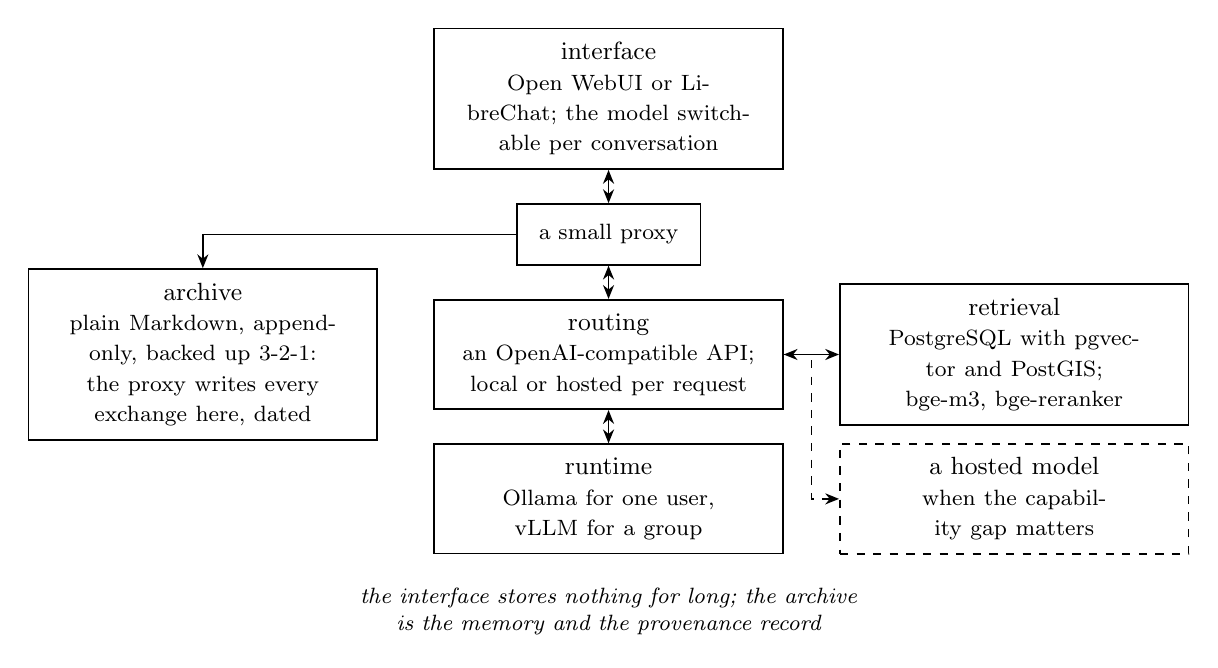
\begin{tikzpicture}[node distance=12pt and 20pt, part/.style={box, text width=110pt, align=center}]
  \node[part] (ui) {interface\\ \footnotesize Open WebUI or LibreChat; the model switchable per conversation};
  \node[box, below=of ui, font=\footnotesize] (proxy) {a small proxy};
  \node[part, below=of proxy] (route) {routing\\ \footnotesize an OpenAI-compatible API; local or hosted per request};
  \node[part, below=of route] (rt) {runtime\\ \footnotesize Ollama for one user, vLLM for a group};
  \node[part, right=of route] (ret) {retrieval\\ \footnotesize PostgreSQL with pgvector and PostGIS; bge-m3, bge-reranker};
  \node[part, dashed, right=of rt] (hosted) {a hosted model\\ \footnotesize when the capability gap matters};
  \node[part, left=of route] (arch) {archive\\ \footnotesize plain Markdown, append-only, backed up 3-2-1: the proxy writes every exchange here, dated};
  \draw[<->] (ui) -- (proxy);
  \draw[<->] (proxy) -- (route);
  \draw[<->] (route) -- (rt);
  \draw[<->] (route) -- (ret);
  \draw[->, dashed] (route.east) -- ++(10pt,0) |- (hosted.west);
  \draw[->] (proxy.west) -| (arch.north);
  \node[note, below=10pt of rt, text width=250pt] {the interface stores nothing for long; the archive is the memory and the provenance record};
\end{tikzpicture}
\end{document}
